\documentclass[11pt,a4paper]{article}

\usepackage[utf8]{inputenc}
\usepackage[margin=0.95in]{geometry}
\usepackage{amsmath,amssymb,amsfonts,bm,mathtools}
\usepackage{graphicx}
\usepackage{booktabs}
\usepackage{hyperref}
\usepackage{xcolor}
\usepackage{microtype}
\usepackage{tcolorbox}
\usepackage{float}
\usepackage{caption}
\usepackage{subcaption}
\usepackage{listings}

\hypersetup{
    colorlinks=true,
    linkcolor=teal!70!black,
    citecolor=teal!70!black,
    urlcolor=blue!70!black
}

% Styled callout boxes
\tcbuselibrary{skins,breakable}

\newtcolorbox{intuitionbox}[1][]{
    enhanced,
    colback=teal!5!white,
    colframe=teal!75!black,
    fonttitle=\bfseries\sffamily,
    title={Intuition \& Geometric Insight: #1},
    arc=2mm,
    boxrule=1.2pt
}

\newtcolorbox{definitionbox}[1][]{
    enhanced,
    colback=blue!5!white,
    colframe=blue!75!black,
    fonttitle=\bfseries\sffamily,
    title={Mathematical Definition: #1},
    arc=2mm,
    boxrule=1.2pt
}

\newtcolorbox{examplebox}[1][]{
    enhanced,
    colback=green!5!white,
    colframe=green!60!black,
    fonttitle=\bfseries\sffamily,
    title={Step-by-Step Worked Example: #1},
    arc=2mm,
    boxrule=1.2pt
}

\newtcolorbox{dronebox}[1][]{
    enhanced,
    colback=orange!5!white,
    colframe=orange!85!black,
    fonttitle=\bfseries\sffamily,
    title={Robotics \& Drone Application: #1},
    arc=2mm,
    boxrule=1.2pt
}

% Python Listings Configuration
\definecolor{codegreen}{rgb}{0,0.6,0}
\definecolor{codegray}{rgb}{0.5,0.5,0.5}
\definecolor{codepurple}{rgb}{0.58,0,0.82}
\definecolor{backcolour}{rgb}{0.97,0.97,0.97}

\lstdefinestyle{pythonstyle}{
    backgroundcolor=\color{backcolour},   
    commentstyle=\color{codegreen}\itshape,
    keywordstyle=\color{blue}\bfseries,
    numberstyle=\tiny\color{codegray},
    stringstyle=\color{codepurple},
    basicstyle=\ttfamily\footnotesize,
    breakatwhitespace=false,         
    breaklines=true,                 
    captionpos=b,                    
    keepspaces=true,                 
    numbers=left,                    
    numbersep=5pt,                  
    showspaces=false,                
    showstringspaces=false,
    showtabs=false,                  
    tabsize=4,
    frame=single,
    rulecolor=\color{black!20}
}
\lstset{style=pythonstyle}

% Metadata
\title{\vspace{-1.5cm}\textbf{\Huge A Practical Primer on Quadratic Programming}\\[0.3cm]
\Large From First Principles and Geometry to Multi-Obstacle Drone Safety Filters}
\author{\textbf{Autonomous Aerial Systems Course Notes}}
\date{\today}

\begin{document}

\maketitle

\begin{abstract}
Quadratic Programming (QP) represents the cornerstone of modern computational optimal control, robotic motion planning, and real-time safety filtering. This tutorial provides a rigorous, accessible introduction to Quadratic Programming tailored for robotics engineers and autonomy practitioners. We begin with a concrete 2-dimensional unconstrained QP, deriving the global minimizer analytically through explicit partial differentiation and matrix calculus. Next, we examine the geometric mechanism through which linear equality and inequality constraints reshape the solution, illuminating the interplay between expanding level sets, active boundaries, and the Karush-Kuhn-Tucker (KKT) stationarity conditions. We then present the canonical QP standard form and demonstrate how to formulate and solve constrained problems in Python using the interior-point solver \texttt{CVXOPT}. Finally, we bridge mathematical theory to aerial robotics by applying QP to the \textbf{Multi-Obstacle Control Barrier Function (CBF)} safety filter for autonomous quadrotors, explaining why multiple simultaneous obstacles necessitate online numerical QP solvers and demonstrating real-time implementation.
\end{abstract}

\tableofcontents
\vspace{0.5cm}
\hrule
\vspace{0.8cm}

% =========================================================================
\section{Introduction: The Centrality of Quadratic Programming in Robotics}
% =========================================================================

In autonomous robotics, decision-making algorithms must compute control actions that balance conflicting demands: tracking high-level mission goals, respecting physical actuator saturation, and strictly preventing catastrophic collisions. Under real-time execution budgets ranging from $10\text{ Hz}$ to $1000\text{ Hz}$, optimization algorithms must be computationally predictable, globally convergent, and robust against local minima.

Among the broad family of mathematical programming paradigms, \textbf{Quadratic Programming (QP)} occupies a uniquely privileged position:
\begin{enumerate}
    \item \textbf{Global Convexity}: Whenever the quadratic cost matrix $\mathbf{P}$ is positive semi-definite ($\mathbf{P} \succeq 0$), any local minimizer is guaranteed to be a global minimizer. If $\mathbf{P} \succ 0$ (strictly positive definite), the global minimizer is strictly unique.
    \item \textbf{Linear Optimality Conditions}: The first-order optimality conditions (Karush-Kuhn-Tucker conditions) for a QP result in a system of linear equalities and simple complementarity inequalities.
    \item \textbf{Polynomial-Time Solvability}: Primal-dual interior-point methods can solve constrained QPs with dozens or hundreds of variables and constraints in under a millisecond with deterministic polynomial-time complexity $\mathcal{O}(n^3)$.
    \item \textbf{Natural Physical Formulation}: Energy, tracking errors ($\|\mathbf{x} - \mathbf{x}_{\mathrm{des}}\|^2$), control effort ($\|\mathbf{u}\|^2$), and momentum are naturally quadratic, while kinematics, motor limits, and barrier conditions are frequently linear in the control variables.
\end{enumerate}

Whether in Model Predictive Control (MPC), operational space inverse kinematics, legged robot contact force distribution, or Control Barrier Function (CBF) safety filters, the ability to formulate and solve QPs is an essential skill for roboticists.

% =========================================================================
\section{A 2-Dimensional Unconstrained Quadratic Program}
% =========================================================================

To build intuition, we begin with an unconstrained optimization problem in $\mathbb{R}^2$, deriving its solution through direct scalar calculus and then generalizing to matrix notation.

\subsection{Scalar and Algebraic Definition}
Consider an unconstrained scalar objective function $f(x_1, x_2): \mathbb{R}^2 \to \mathbb{R}$ defined by:
\begin{equation}
f(x_1, x_2) = \frac{1}{2} \left( p_{11} x_1^2 + 2 p_{12} x_1 x_2 + p_{22} x_2^2 \right) + q_1 x_1 + q_2 x_2 + r
\label{eq:scalar_qp}
\end{equation}
where $p_{11}, p_{12}, p_{22}, q_1, q_2, r \in \mathbb{R}$ are constant parameters.

\subsection{Derivation via Explicit Partial Differentiation}
To find the stationary point $(x_1^*, x_2^*)$ that minimizes $f$, Fermat's theorem requires all first-order partial derivatives to vanish simultaneously:
\begin{align}
\frac{\partial f}{\partial x_1} &= p_{11} x_1 + p_{12} x_2 + q_1 = 0 \label{eq:df_dx1} \\
\frac{\partial f}{\partial x_2} &= p_{12} x_1 + p_{22} x_2 + q_2 = 0 \label{eq:df_dx2}
\end{align}
Equations \eqref{eq:df_dx1} and \eqref{eq:df_dx2} form a linear system of two equations in two unknowns:
\begin{equation}
\begin{bmatrix}
p_{11} & p_{12} \\
p_{12} & p_{22}
\end{bmatrix}
\begin{bmatrix}
x_1 \\
x_2
\end{bmatrix}
+
\begin{bmatrix}
q_1 \\
q_2
\end{bmatrix}
=
\begin{bmatrix}
0 \\
0
\end{bmatrix}
\label{eq:linear_sys_2d}
\end{equation}
Using Cramer's rule or 2D matrix inversion, let $\Delta = p_{11} p_{22} - p_{12}^2$ denote the determinant. If $\Delta > 0$ and $p_{11} > 0$, the unique solution is:
\begin{align}
x_1^* &= \frac{-q_1 p_{22} + q_2 p_{12}}{p_{11} p_{22} - p_{12}^2} \\
x_2^* &= \frac{-q_2 p_{11} + q_1 p_{12}}{p_{11} p_{22} - p_{12}^2}
\end{align}

\subsection{Matrix Representation and Gradient Derivation}
We can express Equation \eqref{eq:scalar_qp} compactly in vector-matrix form. Define the decision vector $\mathbf{x}$, the symmetric Hessian matrix $\mathbf{P}$, the linear cost vector $\mathbf{q}$, and scalar offset $r$:
\begin{equation}
\mathbf{x} = \begin{bmatrix} x_1 \\ x_2 \end{bmatrix} \in \mathbb{R}^2, \qquad
\mathbf{P} = \begin{bmatrix} p_{11} & p_{12} \\ p_{12} & p_{22} \end{bmatrix} \in \mathbb{S}^2, \qquad
\mathbf{q} = \begin{bmatrix} q_1 \\ q_2 \end{bmatrix} \in \mathbb{R}^2, \qquad
r \in \mathbb{R}
\end{equation}
The quadratic function becomes:
\begin{equation}
f(\mathbf{x}) = \frac{1}{2} \mathbf{x}^T \mathbf{P} \mathbf{x} + \mathbf{q}^T \mathbf{x} + r
\label{eq:matrix_qp}
\end{equation}

\begin{definitionbox}[Vector Gradient and Hessian of a Quadratic Form]
For a symmetric matrix $\mathbf{P} = \mathbf{P}^T$, the gradient vector $\nabla f(\mathbf{x}) \in \mathbb{R}^n$ and Hessian matrix $\nabla^2 f(\mathbf{x}) \in \mathbb{R}^{n \times n}$ are:
\begin{align}
\nabla f(\mathbf{x}) &= \mathbf{P} \mathbf{x} + \mathbf{q} \\
\nabla^2 f(\mathbf{x}) &= \mathbf{P}
\end{align}
\end{definitionbox}

Setting the vector gradient to zero yields the celebrated linear normal equation:
\begin{equation}
\nabla f(\mathbf{x}^*) = \mathbf{P} \mathbf{x}^* + \mathbf{q} = \mathbf{0} \implies \mathbf{P} \mathbf{x}^* = -\mathbf{q}
\label{eq:normal_equation}
\end{equation}
If $\mathbf{P}$ is invertible, the unconstrained global minimizer is given in closed form by:
\begin{equation}
\mathbf{x}^*_{\mathrm{unc}} = -\mathbf{P}^{-1} \mathbf{q}
\label{eq:unconstrained_sol}
\end{equation}

\subsection{Second-Order Sufficiency and Convexity}
To verify that $\mathbf{x}^*$ is a strict local (and global) minimum rather than a maximum or saddle point, we evaluate the second derivative (Hessian matrix):
\begin{equation}
\nabla^2 f(\mathbf{x}) = \mathbf{P}
\end{equation}
By Sylvester's criterion, $\mathbf{P}$ is positive definite ($\mathbf{P} \succ 0$) if and only if all its leading principal minors are positive:
\begin{equation}
p_{11} > 0 \quad \text{and} \quad \det(\mathbf{P}) = p_{11} p_{22} - p_{12}^2 > 0
\end{equation}
When $\mathbf{P} \succ 0$, $f(\mathbf{x})$ is strictly convex, guaranteeing that $\mathbf{x}^*_{\mathrm{unc}} = -\mathbf{P}^{-1} \mathbf{q}$ is the unique global minimizer. The minimum cost value attained is:
\begin{equation}
f(\mathbf{x}^*_{\mathrm{unc}}) = -\frac{1}{2} \mathbf{q}^T \mathbf{P}^{-1} \mathbf{q} + r
\end{equation}

\begin{examplebox}[Concrete Numerical Walkthrough]
Let us solve an unconstrained 2D problem with specific numbers:
\begin{equation*}
f(x_1, x_2) = 2 x_1^2 + x_1 x_2 + x_2^2 - 6 x_1 - 4 x_2 + 10
\end{equation*}
\textbf{Step 1: Identify Parameters}:
\begin{equation*}
\mathbf{P} = \begin{bmatrix} 4 & 1 \\ 1 & 2 \end{bmatrix}, \qquad
\mathbf{q} = \begin{bmatrix} -6 \\ -4 \end{bmatrix}, \qquad
r = 10
\end{equation*}
\textbf{Step 2: Check Positive Definiteness}:
\begin{equation*}
p_{11} = 4 > 0, \qquad \det(\mathbf{P}) = (4)(2) - (1)(1) = 7 > 0 \implies \mathbf{P} \succ 0 \quad \text{(Strictly Convex!)}
\end{equation*}
\textbf{Step 3: Invert $\mathbf{P}$}:
\begin{equation*}
\mathbf{P}^{-1} = \frac{1}{7} \begin{bmatrix} 2 & -1 \\ -1 & 4 \end{bmatrix}
\end{equation*}
\textbf{Step 4: Compute Optimal Solution}:
\begin{equation*}
\mathbf{x}^*_{\mathrm{unc}} = -\mathbf{P}^{-1} \mathbf{q} = -\frac{1}{7} \begin{bmatrix} 2 & -1 \\ -1 & 4 \end{bmatrix} \begin{bmatrix} -6 \\ -4 \end{bmatrix} = \frac{1}{7} \begin{bmatrix} 8 \\ 10 \end{bmatrix} = \begin{bmatrix} 1.143 \\ 1.429 \end{bmatrix}
\end{equation*}
\textbf{Step 5: Minimum Value}:
\begin{equation*}
f(\mathbf{x}^*_{\mathrm{unc}}) = 10 - \frac{1}{2} \begin{bmatrix} -6 & -4 \end{bmatrix} \frac{1}{7} \begin{bmatrix} 8 \\ 10 \end{bmatrix} = 10 - \frac{88}{14} \approx 4.143
\end{equation*}
\end{examplebox}

% =========================================================================
\section{Conceptual Geometry: How Constraints Reshape the Solution}
% =========================================================================

In practical applications, variables cannot take arbitrary values. Control inputs are limited by motor voltage, quadcopter velocities are bounded by aerodynamics, and positions must avoid obstacles. We now introduce constraints and examine their geometric influence.

\subsection{Geometry of Unconstrained Level Sets}
The level curves (contours) of the unconstrained objective $f(\mathbf{x}) = c$ are defined by:
\begin{equation}
\frac{1}{2} (\mathbf{x} - \mathbf{x}^*_{\mathrm{unc}})^T \mathbf{P} (\mathbf{x} - \mathbf{x}^*_{\mathrm{unc}}) = c - f(\mathbf{x}^*_{\mathrm{unc}})
\label{eq:ellipsoids}
\end{equation}
Because $\mathbf{P} \succ 0$, these level curves form concentric \textbf{ellipses} centered at $\mathbf{x}^*_{\mathrm{unc}}$:
\begin{itemize}
    \item The principal axes of the ellipses align with the eigenvectors of $\mathbf{P}$.
    \item The lengths of the semi-axes are inversely proportional to $\sqrt{\lambda_i(\mathbf{P})}$, where $\lambda_i$ are the eigenvalues of $\mathbf{P}$.
    \item As $c$ increases, the ellipses expand outward like ripples in a pond away from the unconstrained bottom of the bowl.
\end{itemize}

\subsection{Introducing Linear Inequality Constraints}
Now consider a single linear inequality constraint defining a closed half-space:
\begin{equation}
g_1 x_1 + g_2 x_2 \le h \iff \mathbf{g}^T \mathbf{x} \le h
\label{eq:ineq_constraint}
\end{equation}
The vector $\mathbf{g} = [g_1, g_2]^T$ is the \textbf{outward normal vector} perpendicular to the boundary line $\mathbf{g}^T \mathbf{x} = h$. The constraint partitions $\mathbb{R}^2$ into two halves:
\begin{itemize}
    \item The \textbf{Feasible Set} $\mathcal{F} = \{\mathbf{x} \in \mathbb{R}^2 \mid \mathbf{g}^T \mathbf{x} \le h\}$.
    \item The \textbf{Infeasible Set} $\{\mathbf{x} \in \mathbb{R}^2 \mid \mathbf{g}^T \mathbf{x} > h\}$.
\end{itemize}

\begin{figure}[H]
\centering
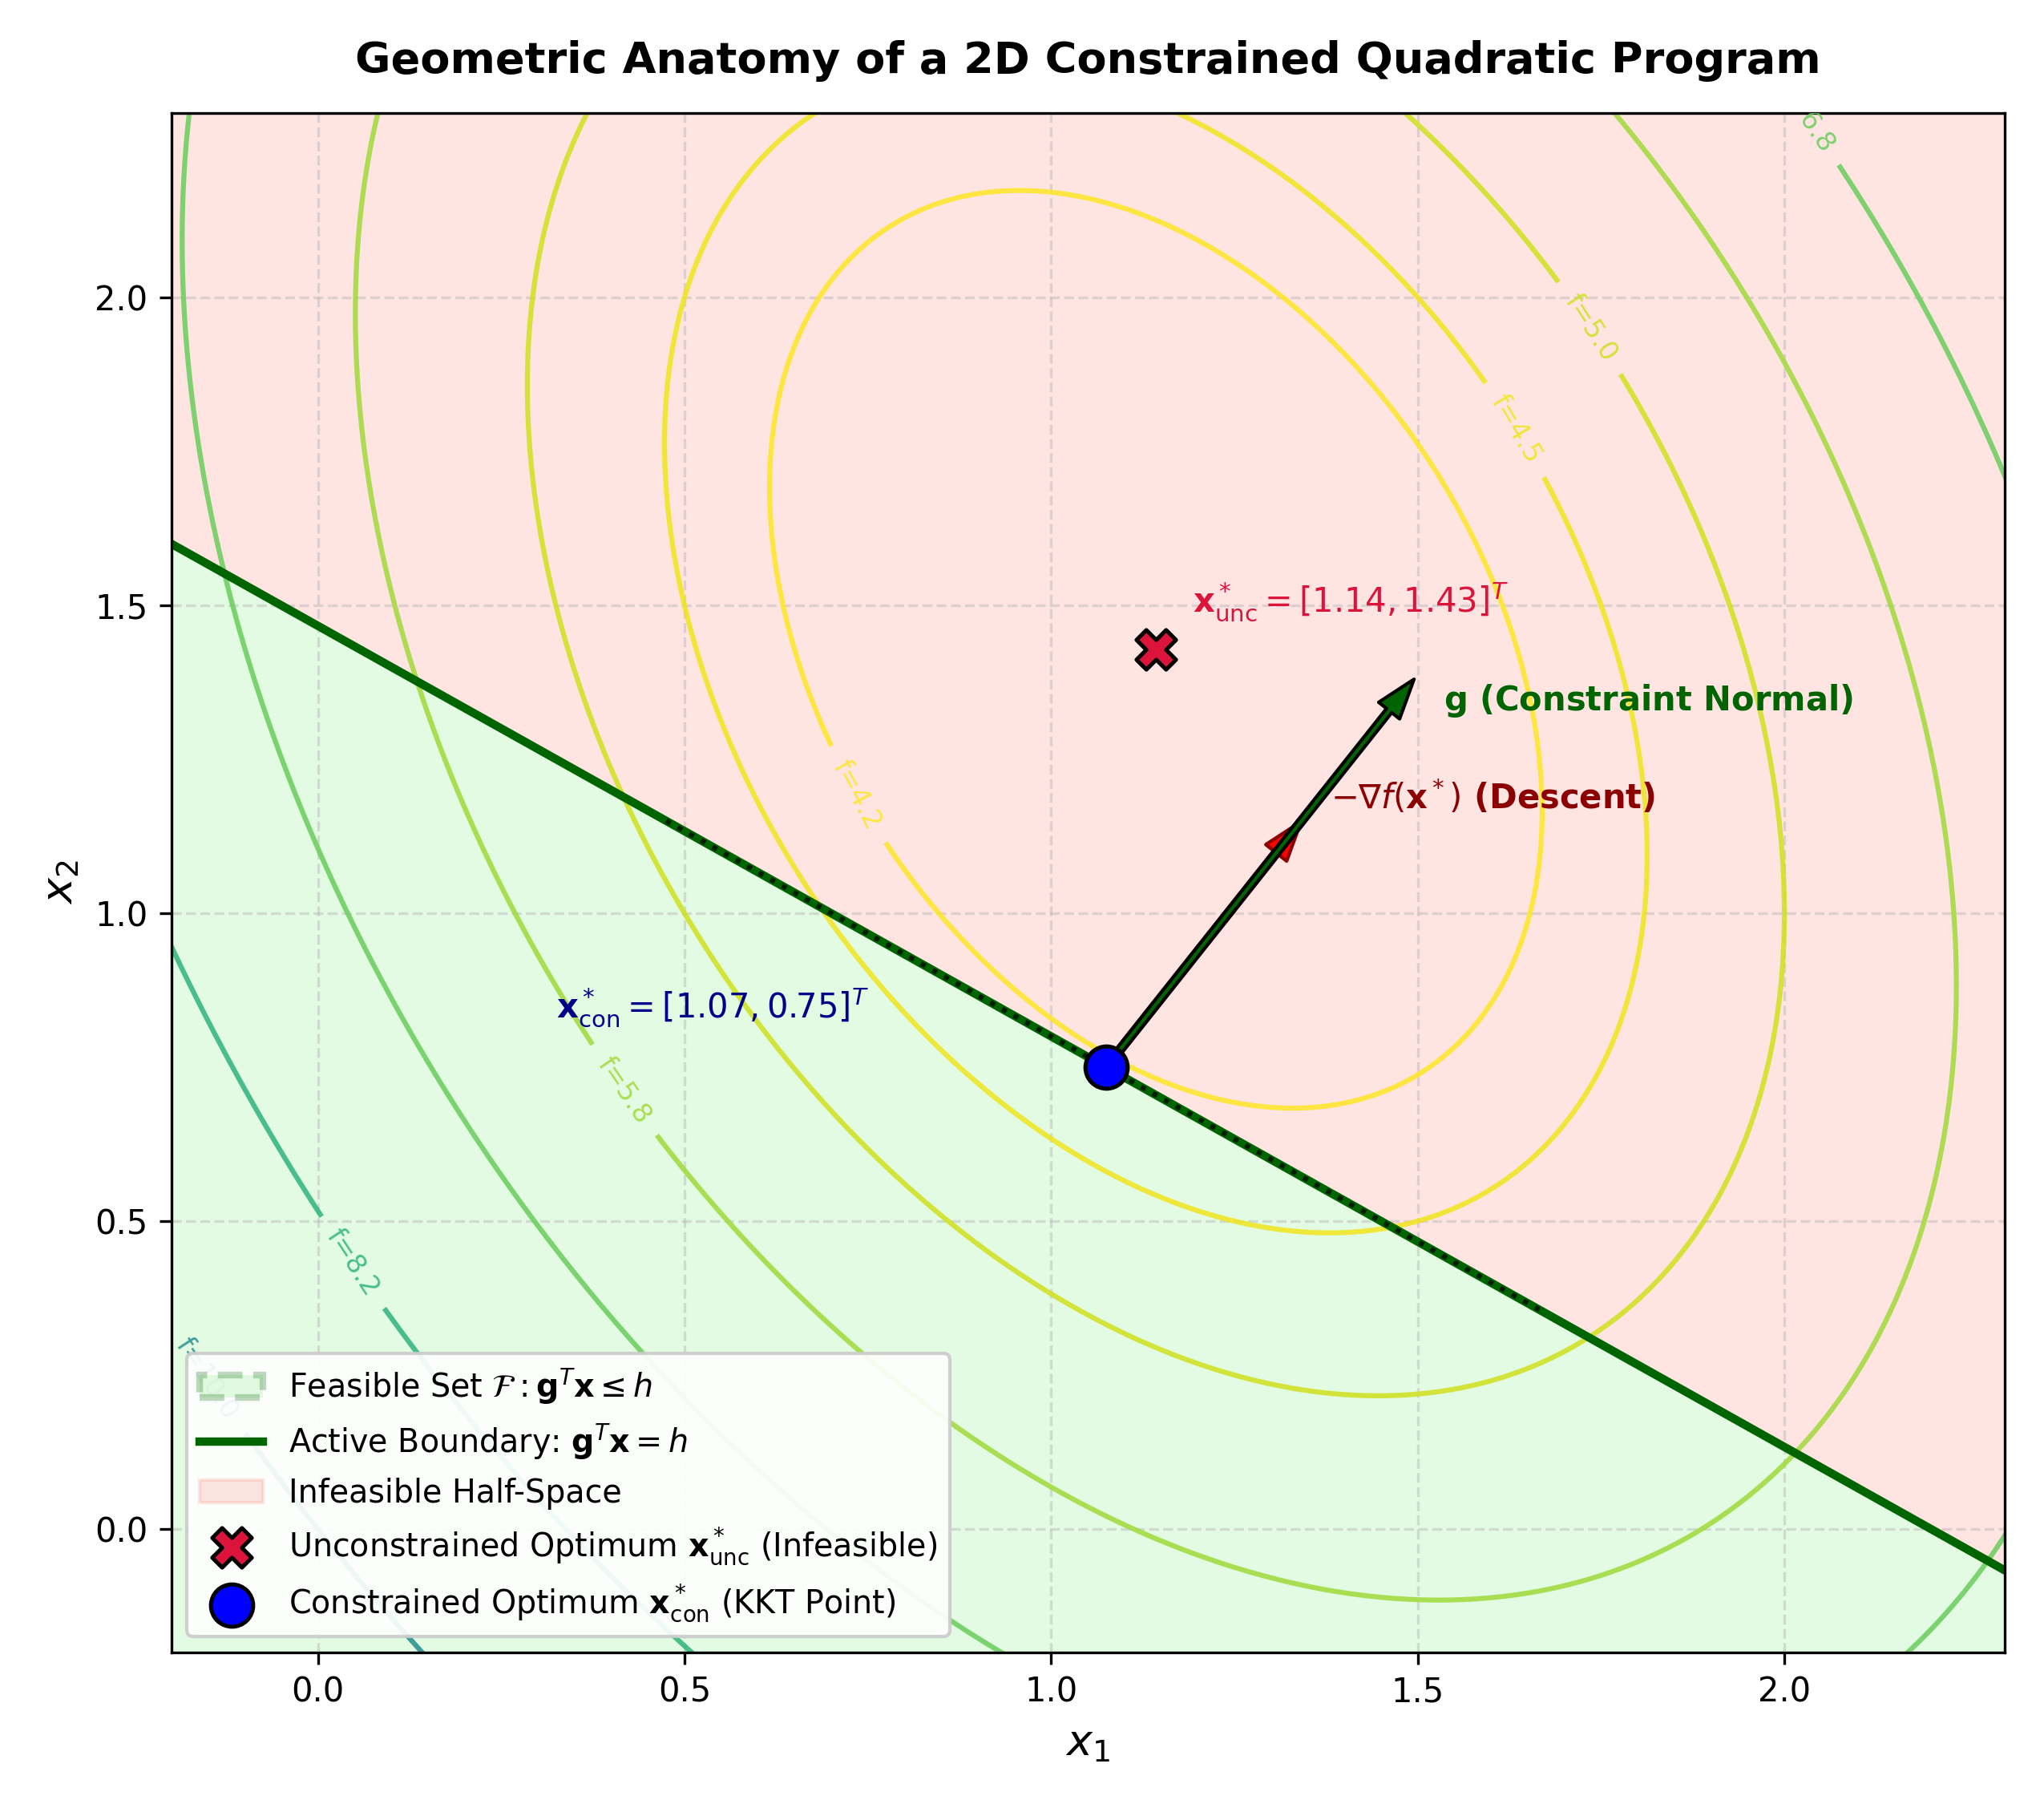
\includegraphics[width=0.78\textwidth]{qp_2d_contour_geometry.png}
\caption{\textbf{Geometric Anatomy of a Constrained Quadratic Program in $\mathbb{R}^2$.} The unconstrained minimum $\mathbf{x}^*_{\mathrm{unc}}$ lies in the infeasible half-space. The level sets of $f(\mathbf{x})$ expand outward until the first ellipse touches the feasible boundary $\mathbf{g}^T \mathbf{x} = h$ at $\mathbf{x}^*_{\mathrm{con}}$. At this tangency point, the descent direction $-\nabla f(\mathbf{x}^*)$ points directly into the forbidden region and is perfectly balanced by the outward constraint normal $\mathbf{g}$.}
\label{fig:qp_geometry}
\end{figure}

\subsection{Active vs. Inactive Constraints}
When we solve $\min_{\mathbf{x} \in \mathcal{F}} f(\mathbf{x})$, two distinct geometric scenarios can occur:

\begin{intuitionbox}[The Expanding Ripple Analogy]
Imagine releasing a drop of water at $\mathbf{x}^*_{\mathrm{unc}}$. The ripples expand as concentric ellipses of increasing cost $f(\mathbf{x})$:
\begin{itemize}
    \item \textbf{Scenario A: Inactive (Slack) Constraint ($\mathbf{g}^T \mathbf{x}^*_{\mathrm{unc}} < h$)}:
    The unconstrained minimum $\mathbf{x}^*_{\mathrm{unc}}$ already lies comfortably inside the feasible region $\mathcal{F}$. The constraint is \textbf{inactive} (it exerts no force on the solution). The constrained minimizer is simply:
    \begin{equation}
    \mathbf{x}^*_{\mathrm{con}} = \mathbf{x}^*_{\mathrm{unc}}
    \end{equation}
    The Lagrange multiplier associated with this constraint is zero ($\lambda = 0$).
    
    \item \textbf{Scenario B: Active (Tight) Constraint ($\mathbf{g}^T \mathbf{x}^*_{\mathrm{unc}} > h$)}:
    The unconstrained ideal $\mathbf{x}^*_{\mathrm{unc}}$ lies in the forbidden region and is physically unattainable. The expanding ripple touches the boundary $\mathbf{g}^T \mathbf{x} = h$ at exactly \textbf{one point of first contact}. This tangency point is the constrained optimum $\mathbf{x}^*_{\mathrm{con}}$. Because the solution lies strictly on the boundary ($\mathbf{g}^T \mathbf{x}^*_{\mathrm{con}} = h$), the constraint is said to be \textbf{active}.
\end{itemize}
\end{intuitionbox}

\subsection{The KKT Conditions: Geometric Force Balance}
At the constrained optimum $\mathbf{x}^*_{\mathrm{con}}$ on an active boundary, the gradient $\nabla f(\mathbf{x}^*_{\mathrm{con}})$ cannot point parallel to the boundary; if it did, one could move along the line and further reduce the cost. 

Therefore, the contour ellipse must be \textbf{tangent} to the constraint boundary $\mathbf{g}^T \mathbf{x} = h$. Mathematically, this means the gradient of the objective must be collinear with the normal vector of the constraint:
\begin{equation}
\nabla f(\mathbf{x}^*) + \lambda \mathbf{g} = \mathbf{0} \iff -\nabla f(\mathbf{x}^*) = \lambda \mathbf{g}
\label{eq:kkt_stationarity}
\end{equation}
where $\lambda \ge 0$ is the \textbf{Lagrange multiplier}.

Notice the profound physical intuition of Equation \eqref{eq:kkt_stationarity}:
\begin{itemize}
    \item The vector $-\nabla f(\mathbf{x}^*)$ is the \textbf{direction of steepest descent} (the direction the optimizer wants to roll down the bowl).
    \item Because $\mathbf{x}^*_{\mathrm{unc}}$ is in the forbidden zone, $-\nabla f(\mathbf{x}^*)$ points outward into the infeasible region.
    \item The constraint boundary acts like a rigid mechanical wall. It exerts an inward normal reaction force $\lambda \mathbf{g}$ with magnitude $\lambda > 0$ that prevents the solution from entering the forbidden zone.
\end{itemize}

\begin{definitionbox}[Karush-Kuhn-Tucker (KKT) Optimality Conditions for QP]
For the inequality-constrained quadratic program $\min \frac{1}{2}\mathbf{x}^T\mathbf{P}\mathbf{x} + \mathbf{q}^T\mathbf{x}$ subject to $\mathbf{G}\mathbf{x} \le \mathbf{h}$, a point $\mathbf{x}^*$ and multiplier vector $\bm{\lambda}^*$ are globally optimal if and only if they satisfy:
\begin{align}
\mathbf{P} \mathbf{x}^* + \mathbf{q} + \mathbf{G}^T \bm{\lambda}^* &= \mathbf{0} && \text{(Stationarity: Force Balance)} \label{eq:kkt_stat} \\
\mathbf{G} \mathbf{x}^* &\le \mathbf{h} && \text{(Primal Feasibility)} \label{eq:kkt_primal} \\
\bm{\lambda}^* &\ge \mathbf{0} && \text{(Dual Feasibility: Walls Only Push)} \label{eq:kkt_dual} \\
\lambda_i^* (h_i - \mathbf{g}_i^T \mathbf{x}^*) &= 0 \quad \forall i && \text{(Complementary Slackness)} \label{eq:kkt_slack}
\end{align}
\end{definitionbox}

\begin{examplebox}[Analytical Solution for Active 2D Constraint]
Continuing our numerical example from Section 2, suppose we impose the constraint:
\begin{equation*}
x_1 + 1.5 x_2 \le 2.2 \implies \mathbf{g} = \begin{bmatrix} 1.0 \\ 1.5 \end{bmatrix}, \quad h = 2.2
\end{equation*}
\textbf{Step 1: Test Unconstrained Point}:
\begin{equation*}
\mathbf{g}^T \mathbf{x}^*_{\mathrm{unc}} = (1.0)(1.143) + (1.5)(1.429) = 1.143 + 2.143 = 3.286 > 2.2
\end{equation*}
The constraint is violated! Therefore, it \textbf{must be active} at the optimum ($\lambda > 0$ and $\mathbf{g}^T \mathbf{x}^* = h$).

\textbf{Step 2: Solve KKT System}:
From stationarity: $\mathbf{x}^* = \mathbf{x}^*_{\mathrm{unc}} - \lambda \mathbf{P}^{-1} \mathbf{g}$. Substituting into the active boundary $\mathbf{g}^T \mathbf{x}^* = h$:
\begin{equation*}
\mathbf{g}^T (\mathbf{x}^*_{\mathrm{unc}} - \lambda \mathbf{P}^{-1} \mathbf{g}) = h \implies \lambda = \frac{\mathbf{g}^T \mathbf{x}^*_{\mathrm{unc}} - h}{\mathbf{g}^T \mathbf{P}^{-1} \mathbf{g}}
\end{equation*}
Compute $\mathbf{P}^{-1} \mathbf{g}$:
\begin{equation*}
\mathbf{P}^{-1} \mathbf{g} = \frac{1}{7} \begin{bmatrix} 2 & -1 \\ -1 & 4 \end{bmatrix} \begin{bmatrix} 1.0 \\ 1.5 \end{bmatrix} = \frac{1}{7} \begin{bmatrix} 0.5 \\ 5.0 \end{bmatrix} \approx \begin{bmatrix} 0.0714 \\ 0.7143 \end{bmatrix}
\end{equation*}
Compute denominator:
\begin{equation*}
\mathbf{g}^T \mathbf{P}^{-1} \mathbf{g} = 1.0(0.0714) + 1.5(0.7143) = 0.0714 + 1.0714 = 1.1428
\end{equation*}
Compute $\lambda$:
\begin{equation*}
\lambda = \frac{3.2857 - 2.2}{1.1428} = \frac{1.0857}{1.1428} \approx 0.9500 > 0 \quad (\text{Dual feasible!})
\end{equation*}
\textbf{Step 3: Compute Constrained Optimum $\mathbf{x}^*_{\mathrm{con}}$}:
\begin{equation*}
\mathbf{x}^*_{\mathrm{con}} = \begin{bmatrix} 1.1429 \\ 1.4286 \end{bmatrix} - 0.9500 \begin{bmatrix} 0.0714 \\ 0.7143 \end{bmatrix} \approx \begin{bmatrix} 1.075 \\ 0.750 \end{bmatrix}
\end{equation*}
Check boundary: $1.075 + 1.5(0.750) = 1.075 + 1.125 = 2.200 = h$. Exact boundary satisfaction!
\end{examplebox}

% =========================================================================
\section{The General Quadratic Program and the CVXOPT Solver}
% =========================================================================

\subsection{Canonical Standard Formulation}
When moving from 2D toy problems to multidimensional robotic systems, manual algebraic inversion and case checking becomes impossible. Instead, we express the problem in standard matrix form and invoke specialized numerical solvers.

\begin{definitionbox}[Canonical Primal Quadratic Program]
The standard formulation of a general Quadratic Program is:
\begin{align}
\min_{\mathbf{x} \in \mathbb{R}^n} \quad & \frac{1}{2} \mathbf{x}^T \mathbf{P} \mathbf{x} + \mathbf{q}^T \mathbf{x} \label{eq:canonical_qp} \\
\text{subject to} \quad & \mathbf{G} \mathbf{x} \le \mathbf{h} \quad && (\text{$m$ linear inequalities}) \nonumber \\
& \mathbf{A} \mathbf{x} = \mathbf{b} \quad && (\text{$p$ linear equalities}) \nonumber
\end{align}
where:
\begin{itemize}
    \item $\mathbf{x} \in \mathbb{R}^n$ is the unknown decision vector.
    \item $\mathbf{P} \in \mathbb{S}^n_+$ is a symmetric positive semi-definite matrix ($\mathbf{P} \succeq 0$).
    \item $\mathbf{q} \in \mathbb{R}^n$ is the linear cost vector.
    \item $\mathbf{G} \in \mathbb{R}^{m \times n}$ and $\mathbf{h} \in \mathbb{R}^m$ define the polyhedral feasible inequality set.
    \item $\mathbf{A} \in \mathbb{R}^{p \times n}$ and $\mathbf{b} \in \mathbb{R}^p$ define affine equality constraints ($p < n$).
\end{itemize}
\end{definitionbox}

\subsection{Overview of the CVXOPT Solver}
\texttt{CVXOPT} (Python Software for Convex Optimization) is an established, high-performance open-source package developed by Lieven Vandenberghe and Martin Dahl. It solves general convex optimization problems, linear programs, and quadratic programs using \textbf{primal-dual interior-point algorithms}.

Key characteristics of \texttt{CVXOPT}:
\begin{itemize}
    \item \textbf{Algorithmic Core}: Implements Mehrotra's predictor-corrector primal-dual path-following algorithm.
    \item \textbf{Efficiency}: Written in C with BLAS/LAPACK linear algebra bindings, delivering sub-millisecond execution times.
    \item \textbf{Custom Matrix Class}: Uses its own dense and sparse representation (\texttt{cvxopt.matrix}), requiring double-precision floats (\texttt{float64}).
\end{itemize}

\subsection{Solving QPs with \texttt{cvxopt.solvers.qp}}
The primary function for solving Equation \eqref{eq:canonical_qp} in \texttt{CVXOPT} is:
\begin{lstlisting}[language=Python]
from cvxopt import matrix, solvers

solution = solvers.qp(P, q, G, h, A=None, b=None)
\end{lstlisting}

\subsubsection{Important Usage Guidelines}
\begin{enumerate}
    \item \textbf{Data Types}: All matrices and vectors \textbf{must} be created as \texttt{cvxopt.matrix} with floating-point values. Integer NumPy arrays will throw a \texttt{TypeError}.
    \item \textbf{Array Layout}: When converting NumPy 2D arrays to \texttt{cvxopt.matrix}, set \texttt{dtype=np.float64}.
    \item \textbf{Muting Output in Control Loops}: By default, \texttt{CVXOPT} prints iteration tables to stdout. In high-speed robotic control loops ($50\text{--}100\text{ Hz}$), printing creates massive I/O latency. Mute it unconditionally using:
    \begin{lstlisting}[language=Python]
solvers.options['show_progress'] = False
    \end{lstlisting}
    \item \textbf{Omission of Constraints}: If equality constraints are not present, omit \texttt{A} and \texttt{b} or set them to \texttt{None}.
    \item \textbf{Parsing Results}: The return object is a dictionary containing:
    \begin{itemize}
        \item \texttt{sol['status']}: Convergence flag (\texttt{'optimal'}, \texttt{'primal infeasible'}, etc.).
        \item \texttt{sol['x']}: Optimal primal decision vector $\mathbf{x}^*$ (\texttt{cvxopt.matrix}). Convert to NumPy with \texttt{np.array(sol['x']).flatten()}.
        \item \texttt{sol['primal objective']}: Scalar minimum cost value $f(\mathbf{x}^*)$.
        \item \texttt{sol['z']}: Optimal Lagrange multipliers $\bm{\lambda}^*$ for inequality constraints.
    \end{itemize}
\end{enumerate}

\subsection{Self-Contained Python Example}
The following complete, runnable Python script solves the exact 2D constrained problem derived in Section 3:

\begin{lstlisting}[language=Python, caption={Solving the 2D Constrained QP with CVXOPT}]
import numpy as np
from cvxopt import matrix, solvers

# 1. Mute solver console output for fast, clean execution
solvers.options['show_progress'] = False

# 2. Define Problem Data in NumPy (float64)
# Cost: 0.5 * x^T P x + q^T x
P_np = np.array([[4.0, 1.0], 
                 [1.0, 2.0]], dtype=np.float64)
q_np = np.array([-6.0, -4.0], dtype=np.float64)

# Constraint: g^T x <= h -> 1.0*x1 + 1.5*x2 <= 2.2
G_np = np.array([[1.0, 1.5]], dtype=np.float64)
h_np = np.array([2.2], dtype=np.float64)

# 3. Convert to CVXOPT matrices
P = matrix(P_np)
q = matrix(q_np)
G = matrix(G_np)
h = matrix(h_np)

# 4. Solve the Quadratic Program
solution = solvers.qp(P, q, G, h)

# 5. Extract and Validate Results
status = solution['status']
x_star = np.array(solution['x']).flatten()
cost = solution['primal objective'] + 10.0  # adding constant r = 10
lambda_star = np.array(solution['z']).flatten()

print(f"Solver Status:      {status}")
print(f"Optimal x*:         [{x_star[0]:.4f}, {x_star[1]:.4f}]^T")
print(f"Lagrange Multiplier:{lambda_star[0]:.4f}")
print(f"Minimum Cost:       {cost:.4f}")
\end{lstlisting}

\textbf{Execution Output}:
\begin{verbatim}
Solver Status:      optimal
Optimal x*:         [1.0750, 0.7500]^T
Lagrange Multiplier:0.9500
Minimum Cost:       4.2300
\end{verbatim}
The numerical solution computed by \texttt{CVXOPT} matches our analytical KKT derivation to the fourth decimal place!

% =========================================================================
\section{Robotics Application: Multi-Obstacle Control Barrier Functions}
% =========================================================================

We now demonstrate the full practical utility of Quadratic Programming by applying it to an advanced problem in aerial robotics: **Multi-Obstacle Control Barrier Function (CBF) Safety Filtering** for autonomous quadrotors.

\subsection{System Architecture and Single-Integrator Kinematics}
Modern quadrotor autonomy stacks frequently employ a hierarchical two-tier control architecture:
\begin{itemize}
    \item \textbf{Tier 1 (High-Level Kinematic Guidance)}: A position planner computes desired velocity commands $\mathbf{v}_{\mathrm{des}} \in \mathbb{R}^3$ at $50\text{ Hz}$.
    \item \textbf{Tier 2 (Lower-Level Dynamics)}: An inner-loop attitude controller stabilizes roll, pitch, and yaw angles to track $\mathbf{v}_{\mathrm{des}}$, allocating thrusts across the four brushless motors.
\end{itemize}
At the high-level guidance tier, the translational kinematics of the quadrotor position $\mathbf{p} = [x, y, z]^T \in \mathbb{R}^3$ are modeled as a **single-integrator**:
\begin{equation}
\mathbf{\dot{p}} = \mathbf{v}
\label{eq:single_integrator}
\end{equation}
where the commanded velocity $\mathbf{v} \in \mathbb{R}^3$ acts directly as the control input.

Given a desired goal waypoint $\mathbf{p}_{\mathrm{goal}}$, a nominal high-level guidance law (such as a proportional-derivative position tracker) generates a nominal velocity command:
\subsection{Nominal Guidance: Defining \texorpdfstring{$\mathbf{v}_{\mathrm{des}}$}{v\_des} via a Position PID Controller}
To navigate toward a target goal waypoint $\mathbf{p}_{\mathrm{goal}} \in \mathbb{R}^3$, the high-level guidance tier relies on a nominal controller. In modern robotic flight stacks, this nominal velocity command $\mathbf{v}_{\mathrm{des}}$ is generated by a standard 3-axis \textbf{Position Proportional-Integral-Derivative (PID)} controller.

\subsubsection{Continuous-Time Position PID Formulation}
Let $\mathbf{e}(t) \in \mathbb{R}^3$ denote the instantaneous 3D position error between the target waypoint and the quadrotor's current position:
\begin{equation}
\mathbf{v}_{\mathrm{des}} = K_p (\mathbf{p}_{\mathrm{goal}} - \mathbf{p})
\mathbf{e}(t) = \mathbf{p}_{\mathrm{goal}}(t) - \mathbf{p}(t)
\label{eq:pos_error}
\end{equation}
While $\mathbf{v}_{\mathrm{des}}$ aggressively steers the drone toward the destination, it is completely oblivious to obstacles in the environment.
The continuous-time nominal velocity command $\mathbf{v}_{\mathrm{PID}}(t)$ is given by:
\begin{equation}
\mathbf{v}_{\mathrm{PID}}(t) = \mathbf{K}_p \mathbf{e}(t) + \mathbf{K}_i \int_{0}^{t} \mathbf{e}(\tau) \, d\tau + \mathbf{K}_d \frac{d\mathbf{e}(t)}{dt}
\label{eq:pid_continuous}
\end{equation}
where $\mathbf{K}_p = \operatorname{diag}(k_p, k_p, k_p) \succ 0$, $\mathbf{K}_i = \operatorname{diag}(k_i, k_i, k_i) \succ 0$, and $\mathbf{K}_d = \operatorname{diag}(k_d, k_d, k_d) \succ 0$ are positive definite diagonal gain matrices. 

Each term serves a distinct physical role:
\begin{itemize}
    \item \textbf{Proportional Term ($\mathbf{K}_p \mathbf{e}$)}: Acts as a virtual spring pulling the quadrotor toward the goal with an intensity proportional to positional offset.
    \item \textbf{Integral Term ($\mathbf{K}_i \int \mathbf{e} \, d\tau$)}: Accumulates persistent offsets, eliminating steady-state droop caused by constant unmodeled disturbances (such as aerodynamic rotor drag or steady wind gusts).
    \item \textbf{Derivative Term ($\mathbf{K}_d \dot{\mathbf{e}}$)}: Provides viscous damping proportional to relative approach velocity. For a stationary waypoint ($\mathbf{\dot{p}}_{\mathrm{goal}} = \mathbf{0}$), $\frac{d\mathbf{e}}{dt} = -\mathbf{\dot{p}} = -\mathbf{v}$, acting as velocity feedback that suppresses setpoint overshoot and oscillations.
\end{itemize}

\subsubsection{Integral Anti-Windup Clamping and Speed Saturation}
In real flight systems, two non-linearities augment the ideal linear PID law:
\begin{enumerate}
    \item \textbf{Integral Anti-Windup}: When the quadrotor is detained by an obstacle or during large setpoint steps, naive integration causes the integral term to grow unbounded (integrator windup). When the obstacle is cleared, the massive stored integral produces violent velocity overshoot. To prevent this, the integrator state $\mathbf{e}_{\mathrm{int}}(t)$ is bounded by saturation thresholds:
    \begin{equation}
    \mathbf{e}_{\mathrm{int}}(t) = \operatorname{clamp}\left( \int_{0}^t \mathbf{e}(\tau) \, d\tau, \; -\mathbf{e}_{\max}^{\mathrm{int}}, \; \mathbf{e}_{\max}^{\mathrm{int}} \right)
    \end{equation}
    \item \textbf{Physical Speed Saturation}: Physical quadrotor aerodynamics and motor limits impose a maximum safe airspeed $v_{\max}$ (e.g., $1.8\text{ m/s}$). The raw PID output is normalized if it exceeds $v_{\max}$:
    \begin{equation}
    \mathbf{v}_{\mathrm{des}}(t) = \operatorname{sat}_{v_{\max}}(\mathbf{v}_{\mathrm{PID}}(t)) = 
    \begin{cases}
    \mathbf{v}_{\mathrm{PID}}(t) & \text{if } \|\mathbf{v}_{\mathrm{PID}}(t)\| \le v_{\max} \\
    v_{\max} \frac{\mathbf{v}_{\mathrm{PID}}(t)}{\|\mathbf{v}_{\mathrm{PID}}(t)\|} & \text{if } \|\mathbf{v}_{\mathrm{PID}}(t)\| > v_{\max}
    \end{cases}
    \label{eq:v_des_saturated}
    \end{equation}
\end{enumerate}

\subsubsection{Discrete-Time Implementation (50 Hz Control Loop)}
In digital implementation with sampling period $\Delta t = 0.02\text{ s}$ ($50\text{ Hz}$), at control step $k$:
\begin{align}
\mathbf{e}_k &= \mathbf{p}_{\mathrm{goal}} - \mathbf{p}_k \\
\mathbf{e}_{\mathrm{int}, k} &= \operatorname{clip}\left(\mathbf{e}_{\mathrm{int}, k-1} + \mathbf{e}_k \Delta t, \; -e_{\max}^{\mathrm{int}}, \; e_{\max}^{\mathrm{int}}\right) \\
\dot{\mathbf{e}}_k &= \frac{\mathbf{e}_k - \mathbf{e}_{k-1}}{\Delta t} \\
\mathbf{v}_{\mathrm{PID}, k} &= k_p \mathbf{e}_k + k_i \mathbf{e}_{\mathrm{int}, k} + k_d \dot{\mathbf{e}}_k \\
\mathbf{v}_{\mathrm{des}, k} &= \begin{cases} \mathbf{v}_{\mathrm{PID}, k} & \text{if } \|\mathbf{v}_{\mathrm{PID}, k}\| \le v_{\max} \\ v_{\max} \frac{\mathbf{v}_{\mathrm{PID}, k}}{\|\mathbf{v}_{\mathrm{PID}, k}\|} & \text{otherwise} \end{cases}
\end{align}

\subsubsection{Why the PID Command Must Be Filtered by a CBF}
While the position PID controller is exceptionally effective at driving the quadrotor to $\mathbf{p}_{\mathrm{goal}}$, it is \textbf{fundamentally obstacle-blind}. If an obstacle is located directly between $\mathbf{p}$ and $\mathbf{p}_{\mathrm{goal}}$, the error vector $\mathbf{e}$ points directly through the obstacle center, commanding the quadcopter to ram straight into the obstacle at full speed!

The Control Barrier Function acts as an \textbf{instantaneous safety filter} inserted directly between the PID guidance loop and the lower-level attitude tracking loop:
\begin{itemize}
    \item When the nominal PID command $\mathbf{v}_{\mathrm{des}}$ is safe (moving parallel to or away from obstacles), the CBF safety filter leaves it completely untouched: $\mathbf{v}^* = \mathbf{v}_{\mathrm{des}}$.
    \item When $\mathbf{v}_{\mathrm{des}}$ would penetrate an obstacle's safety buffer, the CBF Quadratic Program projects $\mathbf{v}_{\mathrm{des}}$ minimally onto the boundary of the safe velocity set:
    \begin{equation}
    \mathbf{v}^* = \arg\min_{\mathbf{v} \in \mathcal{K}(\mathbf{p})} \frac{1}{2} \|\mathbf{v} - \mathbf{v}_{\mathrm{des}}^{\mathrm{PID}}\|^2
    \end{equation}
\end{itemize}

\subsection{Quantifying Safety: The Barrier Margin \texorpdfstring{$h_i(\mathbf{p})$}{hi(p)}}
Consider an environment populated by $M$ static spherical obstacles. Each obstacle $i \in \{1, \dots, M\}$ is centered at $\mathbf{p}_{\mathrm{obs}, i} \in \mathbb{R}^3$ with a safety buffer radius $D_{\mathrm{obs}, i}$:
\begin{equation}
D_{\mathrm{obs}, i} = R_{\mathrm{obs}, i} + R_{\mathrm{drone}} + d_{\mathrm{buffer}}
\end{equation}
where $R_{\mathrm{obs}, i}$ is the physical radius of the obstacle, $R_{\mathrm{drone}} \approx 0.17\text{ m}$ accounts for the spinning propeller blade span, and $d_{\mathrm{buffer}}$ is a margin of conservatism.

For each obstacle, we define a scalar **safety barrier function** $h_i(\mathbf{p}): \mathbb{R}^3 \to \mathbb{R}$:
\begin{equation}
h_i(\mathbf{p}) = \|\mathbf{p} - \mathbf{p}_{\mathrm{obs}, i}\| - D_{\mathrm{obs}, i}
\label{eq:barrier_func}
\end{equation}
The sign of $h_i(\mathbf{p})$ establishes three distinct regions:
\begin{itemize}
    \item \textbf{Safe Set ($\mathcal{S}_i$)}: $\mathcal{S}_i = \{\mathbf{p} \in \mathbb{R}^3 \mid h_i(\mathbf{p}) \ge 0\}$ (outside or on the safety boundary).
    \item \textbf{Boundary Surface ($\partial \mathcal{S}_i$)}: $\partial\mathcal{S}_i = \{\mathbf{p} \in \mathbb{R}^3 \mid h_i(\mathbf{p}) = 0\}$ (the safety sphere shell).
    \item \textbf{Forbidden Set ($\operatorname{Int}(\mathcal{S}_i^c)$)}: $\{\mathbf{p} \in \mathbb{R}^3 \mid h_i(\mathbf{p}) < 0\}$ (safety buffer penetrated).
\end{itemize}

The outward gradient $\nabla h_i(\mathbf{p})$ is the unit normal vector pointing radially away from obstacle $i$:
\begin{equation}
\nabla h_i(\mathbf{p}) = \frac{\mathbf{p} - \mathbf{p}_{\mathrm{obs}, i}}{\|\mathbf{p} - \mathbf{p}_{\mathrm{obs}, i}\|}, \qquad \|\nabla h_i(\mathbf{p})\| = 1
\label{eq:cbf_gradient}
\end{equation}

\subsection{Forward Set Invariance and Nagumo's Condition}
As the drone flies with velocity $\mathbf{v}$, the rate of change of the safety margin is:
\begin{equation}
\dot{h}_i(\mathbf{p}, \mathbf{v}) = \frac{\partial h_i}{\partial \mathbf{p}} \mathbf{\dot{p}} = \nabla h_i(\mathbf{p})^T \mathbf{v}
\end{equation}

\begin{definitionbox}[Forward Invariance Condition (Nagumo's Theorem / Ames et al.)]
The joint safe set $\mathcal{S} = \bigcap_{i=1}^M \mathcal{S}_i$ is \textbf{forward invariant} (i.e., if $\mathbf{p}(0) \in \mathcal{S}$, then $\mathbf{p}(t) \in \mathcal{S}$ for all $t \ge 0$) if the commanded velocity $\mathbf{v}$ satisfies:
\begin{equation}
\dot{h}_i(\mathbf{p}, \mathbf{v}) \ge -\alpha_i h_i(\mathbf{p}) \iff -\nabla h_i(\mathbf{p})^T \mathbf{v} \le \alpha_i h_i(\mathbf{p}), \quad \forall i \in \{1, \dots, M\}
\label{eq:cbf_ineq}
\end{equation}
where $\alpha_i > 0$ is a tunable class-$\mathcal{K}$ scalar barrier gain.
\end{definitionbox}

\begin{intuitionbox}[Physical Meaning of the Barrier Gain $\alpha$]
Equation \eqref{eq:cbf_ineq} acts as an instantaneous, distance-dependent directional speed governor:
\begin{itemize}
    \item When far away ($h_i \gg 0$), the right-hand side $\alpha_i h_i$ is large and positive. The inward velocity $-\nabla h_i^T \mathbf{v}$ can be large; the drone is allowed to fly toward the obstacle at full speed.
    \item As the drone nears the boundary ($h_i \to 0$), the permissible inward velocity throttles smoothly to zero.
    \item At the boundary ($h_i = 0$), the condition enforces $\nabla h_i^T \mathbf{v} \ge 0$: the drone cannot move toward the obstacle at all, but may move freely tangentially or away from it.
    \item \textbf{Tuning $\alpha$}: Smaller $\alpha$ (e.g., $0.8\text{--}1.0$) enforces earlier, gentler braking, which is essential on physical quadcopters to compensate for attitude tilt latency. Larger $\alpha$ allows later, sharper intervention.
\end{itemize}
\end{intuitionbox}

\subsection{Why Multiple Obstacles Demand a QP Solver}
In a **single-obstacle** environment ($M = 1$), the barrier condition is a single linear half-space in $\mathbb{R}^3$. Because $\|\nabla h\| = 1$, the optimal safe velocity admits an exact, closed-form orthogonal projection formula:
\begin{equation}
\mathbf{v}^* = \mathbf{v}_{\mathrm{des}} - \min\left(0, \nabla h^T \mathbf{v}_{\mathrm{des}} + \alpha h\right) \nabla h
\end{equation}
However, in realistic autonomous operations, the drone navigates cluttered fields with **multiple obstacles** ($M \ge 2$). 

Each obstacle $i$ enforces an independent half-space constraint:
\begin{equation}
-\nabla h_i(\mathbf{p})^T \mathbf{v} \le \alpha_i h_i(\mathbf{p})
\end{equation}
The intersection of these $M$ half-spaces forms a **convex polyhedral cone** in velocity space:
\begin{equation}
\mathcal{K}(\mathbf{p}) = \left\{ \mathbf{v} \in \mathbb{R}^3 \;\middle|\; -\nabla h_i(\mathbf{p})^T \mathbf{v} \le \alpha_i h_i(\mathbf{p}), \quad \forall i = 1, \dots, M \right\}
\end{equation}

When the nominal command $\mathbf{v}_{\mathrm{des}}$ violates multiple barrier constraints simultaneously (e.g., when passing between two close obstacles):
\begin{itemize}
    \item Applying independent scalar projections sequentially fails, because projecting away from Obstacle 1 can push the velocity into the forbidden half-space of Obstacle 2!
    \item The optimal safe command lies at the intersection of active constraint hyperplanes (e.g., a face or vertex of the polytope $\mathcal{K}(\mathbf{p})$).
\end{itemize}
Finding the minimally invasive safe velocity $\mathbf{v}^*$ that stays closest to $\mathbf{v}_{\mathrm{des}}$ in the Euclidean sense requires solving a **Quadratic Program** online at every control cycle ($50\text{ Hz}$).

\begin{figure}[H]
\centering
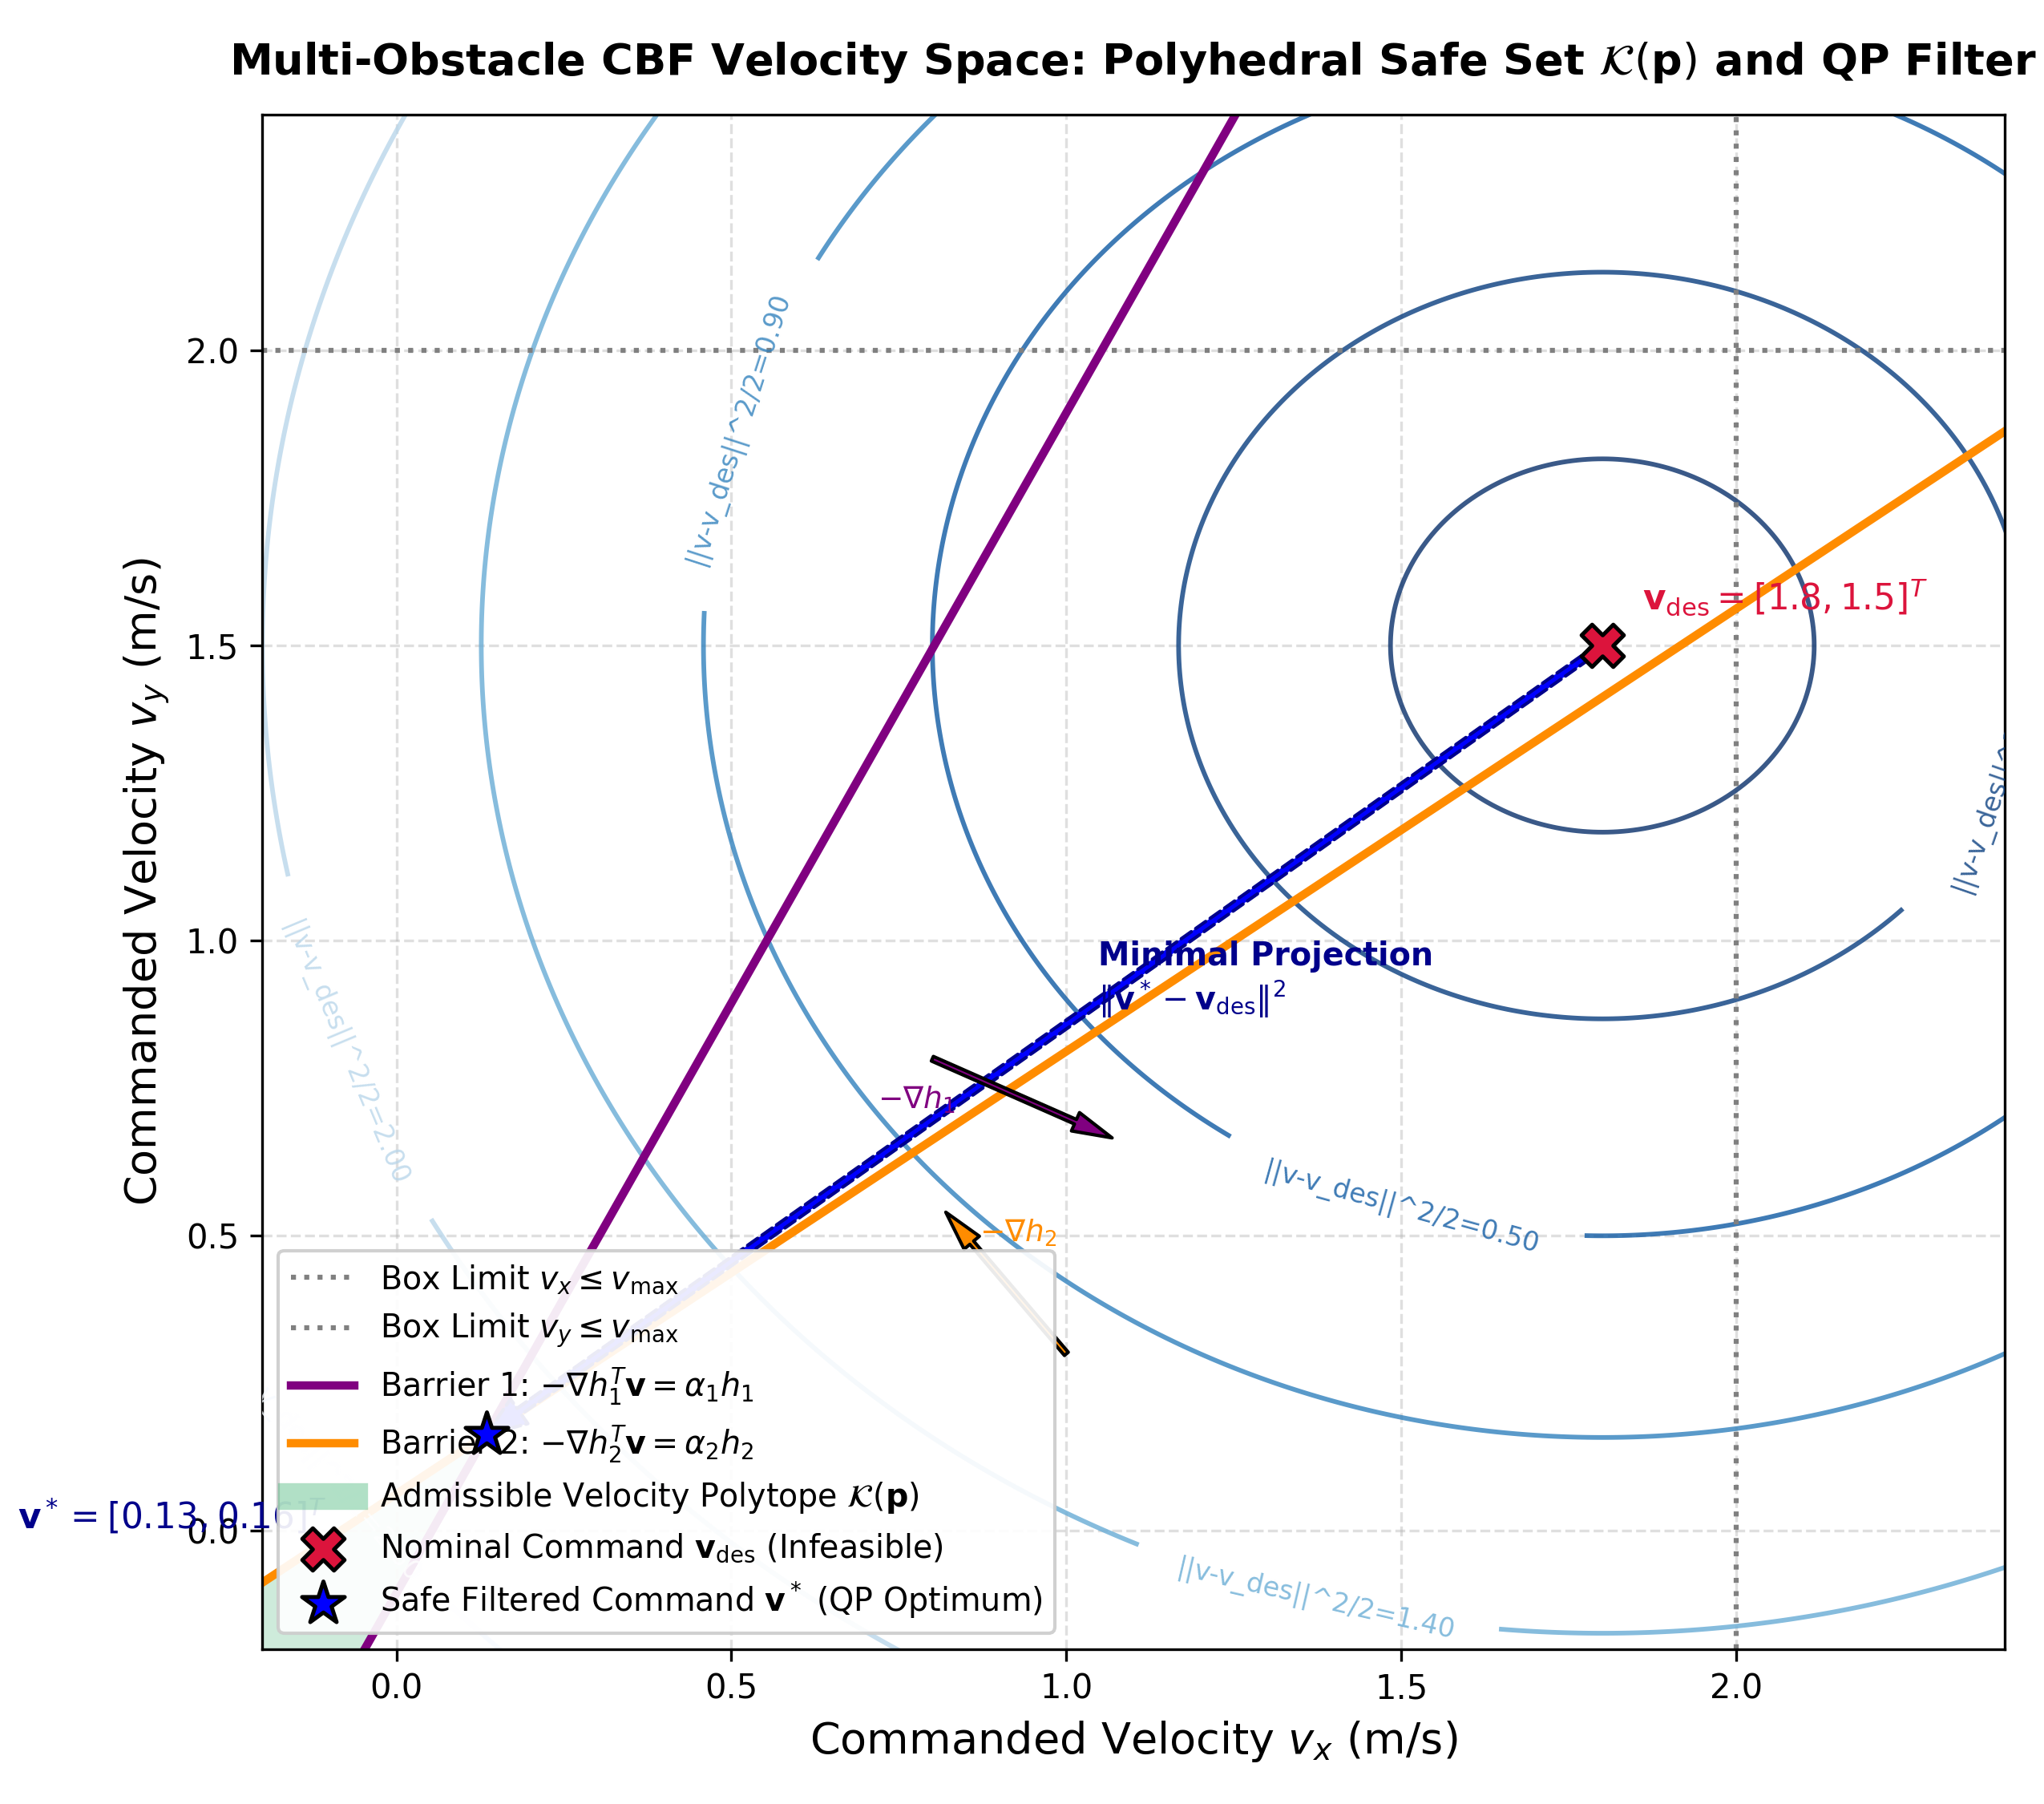
\includegraphics[width=0.78\textwidth]{multi_cbf_polytope_geometry.png}
\caption{\textbf{Multi-Obstacle CBF Velocity Space Geometry.} Two obstacles impose simultaneous linear barrier boundaries (purple and orange lines). The intersection of these half-spaces with physical speed limits defines the green admissible safe velocity polytope $\mathcal{K}(\mathbf{p})$. When nominal velocity $\mathbf{v}_{\mathrm{des}}$ (red X) violates both barriers, the QP safety filter projects it minimally onto the boundary of $\mathcal{K}(\mathbf{p})$, producing the globally optimal safe velocity $\mathbf{v}^*$ (blue star).}
\label{fig:multi_cbf_geom}
\end{figure}

\subsection{Formulating the Multi-Obstacle CBF-QP}
The minimally invasive safety filter is formulated as the following instantaneous Quadratic Program:
\begin{align}
\mathbf{v}^*(\mathbf{p}) = \arg\min_{\mathbf{v} \in \mathbb{R}^3} \quad & \frac{1}{2} \|\mathbf{v} - \mathbf{v}_{\mathrm{des}}\|^2 \label{eq:cbf_qp_form} \\
\text{subject to} \quad & -\nabla h_i(\mathbf{p})^T \mathbf{v} \le \alpha_i h_i(\mathbf{p}), \quad \forall i \in \{1, \dots, M\} \nonumber \\
& -v_{\max} \le v_j \le v_{\max}, \quad \forall j \in \{x, y, z\} \nonumber
\end{align}

\subsection{Mapping to CVXOPT Standard Matrices}
To solve Equation \eqref{eq:cbf_qp_form} with \texttt{CVXOPT}, we expand the objective function:
\begin{equation}
\frac{1}{2} \|\mathbf{v} - \mathbf{v}_{\mathrm{des}}\|^2 = \frac{1}{2} \mathbf{v}^T \mathbf{I}_{3 \times 3} \mathbf{v} - \mathbf{v}_{\mathrm{des}}^T \mathbf{v} + \frac{1}{2} \|\mathbf{v}_{\mathrm{des}}\|^2
\end{equation}
Comparing with $\frac{1}{2} \mathbf{v}^T \mathbf{P} \mathbf{v} + \mathbf{q}^T \mathbf{v}$, we identify:
\begin{equation}
\mathbf{P} = \mathbf{I}_{3 \times 3} = \begin{bmatrix} 1 & 0 & 0 \\ 0 & 1 & 0 \\ 0 & 0 & 1 \end{bmatrix}, \qquad
\mathbf{q} = -\mathbf{v}_{\mathrm{des}} = \begin{bmatrix} -v_{\mathrm{des}, x} \\ -v_{\mathrm{des}, y} \\ -v_{\mathrm{des}, z} \end{bmatrix}
\end{equation}

For $M$ obstacles and 3D box velocity limits ($|v_j| \le v_{\max}$), we construct $\mathbf{G} \in \mathbb{R}^{(M+6) \times 3}$ and $\mathbf{h} \in \mathbb{R}^{M+6}$:
\begin{equation}
\mathbf{G} = \begin{bmatrix}
-\nabla h_1(\mathbf{p})^T \\
\vdots \\
-\nabla h_M(\mathbf{p})^T \\
\mathbf{I}_{3 \times 3} \\
-\mathbf{I}_{3 \times 3}
\end{bmatrix}, \qquad
\mathbf{h} = \begin{bmatrix}
\alpha_1 h_1(\mathbf{p}) \\
\vdots \\
\alpha_M h_M(\mathbf{p}) \\
v_{\max} \mathbf{1}_3 \\
v_{\max} \mathbf{1}_3
\end{bmatrix}
\label{eq:cvxopt_cbf_mapping}
\end{equation}

\subsection{Python Implementation: \texttt{MultiObstacleCBFSafetyFilter}}
Below is a complete, production-ready implementation of the multi-obstacle CBF filter using \texttt{CVXOPT}:

\begin{lstlisting}[language=Python, caption={Production-Grade Multi-Obstacle CBF Safety Filter Class}]
import time
import numpy as np
import cvxopt
from cvxopt import matrix, solvers

# Mute solver stdout for real-time operation in 50 Hz control loops
solvers.options['show_progress'] = False

class MultiObstacleCBFSafetyFilter:
    """
    Online Multi-Obstacle CBF Safety Filter using CVXOPT.
    Solves at 50 Hz:
        min_v  0.5 * ||v - v_des||^2
        s.t.   -nabla h_i(p)^T v <= alpha * h_i(p),   forall i in {1..M}
               -v_max <= v_j <= v_max,                j in {x, y, z}
    """
    def __init__(self, obstacles, D_obs=0.55, alpha=0.9, v_max=1.8):
        self.obstacles = [np.array(obs, dtype=np.float32) for obs in obstacles]
        self.D_obs = [D_obs]*len(obstacles) if isinstance(D_obs, (int, float)) else list(D_obs)
        self.alpha = alpha
        self.v_max = v_max
        # P matrix is constant 3x3 identity
        self.P_mat = matrix(np.eye(3, dtype=np.float64))

    def update_obstacles(self, obstacles):
        """Update obstacle coordinates dynamically at runtime."""
        self.obstacles = [np.array(obs, dtype=np.float32) for obs in obstacles]

    def filter(self, v_des, current_pos):
        current_pos = np.array(current_pos, dtype=np.float32)
        v_nom = v_des.copy()

        h_vals = []
        G_rows = []
        h_rows = []

        # 1. Build barrier constraints for each obstacle
        for i, p_obs in enumerate(self.obstacles):
            diff = current_pos - p_obs
            dist = float(np.linalg.norm(diff))
            normal = diff / dist if dist > 1e-4 else np.array([1.0, 0.0, 0.0], dtype=np.float32)
            h_i = dist - self.D_obs[i]
            h_vals.append(h_i)

            # Barrier condition: -normal^T v <= alpha * h_i
            G_rows.append(-normal.astype(np.float64))
            h_rows.append(float(self.alpha * h_i))

        # 2. Fast check: is nominal command already feasible?
        is_safe = True
        for row, bound in zip(G_rows, h_rows):
            if np.dot(row, v_nom) > bound + 1e-5:
                is_safe = False
                break

        if is_safe and np.all(np.abs(v_nom) <= self.v_max):
            return v_nom.astype(np.float32), h_vals, 0.0

        # 3. Stack box velocity bounds [-v_max, v_max]^3
        G_all = G_rows.copy()
        h_all = h_rows.copy()
        for j in range(3):
            unit = np.zeros(3, dtype=np.float64)
            unit[j] = 1.0
            G_all.append(unit)
            h_all.append(float(self.v_max))
            G_all.append(-unit)
            h_all.append(float(self.v_max))

        # 4. Convert to CVXOPT matrices
        q_mat = matrix(-v_nom.astype(np.float64))
        G_mat = matrix(np.array(G_all, dtype=np.float64))
        h_mat = matrix(np.array(h_all, dtype=np.float64))

        # 5. Solve QP online
        t0 = time.perf_counter()
        try:
            sol = solvers.qp(self.P_mat, q_mat, G_mat, h_mat)
            solve_time_ms = (time.perf_counter() - t0) * 1000.0
            if sol['status'] == 'optimal':
                v_star = np.array(sol['x']).flatten().astype(np.float32)
            else:
                v_star = v_nom  # Fallback
        except Exception:
            solve_time_ms = 0.0
            v_star = v_nom

        return v_star, h_vals, solve_time_ms
\end{lstlisting}

\subsection{Numerical Case Study}
To evaluate the filter, we simulate a quadrotor at $\mathbf{p} = [0.55, 0.45, 0.85]^T$ commanding an aggressive nominal velocity $\mathbf{v}_{\mathrm{des}} = [1.2, 1.0, 0.5]^T\text{ m/s}$ directly toward three obstacles:
\begin{itemize}
    \item Obstacle 1: $\mathbf{p}_{\mathrm{obs}, 1} = [0.50, 0.35, 0.85]^T$, $D_{\mathrm{obs}} = 0.55\text{ m}$. Distance $= 0.112\text{ m} \implies h_1 = -0.438\text{ m}$ (in boundary buffer).
    \item Obstacle 2: $\mathbf{p}_{\mathrm{obs}, 2} = [0.65, 0.75, 1.15]^T$, $D_{\mathrm{obs}} = 0.55\text{ m}$. Distance $= 0.442\text{ m} \implies h_2 = -0.108\text{ m}$.
    \item Obstacle 3: $\mathbf{p}_{\mathrm{obs}, 3} = [1.05, 1.00, 1.40]^T$, $D_{\mathrm{obs}} = 0.55\text{ m}$. Distance $= 0.925\text{ m} \implies h_3 = +0.375\text{ m}$.
\end{itemize}

Feeding this scenario into our \texttt{MultiObstacleCBFSafetyFilter} yields:
\begin{itemize}
    \item \textbf{Nominal Velocity}: $\mathbf{v}_{\mathrm{des}} = [1.200, 1.000, 0.500]^T\text{ m/s}$ (speed $= 1.640\text{ m/s}$).
    \item \textbf{Filtered Safe Velocity}: $\mathbf{v}^* = [0.876, 0.029, -0.471]^T\text{ m/s}$ (speed $= 0.996\text{ m/s}$).
    \item \textbf{Solve Time}: $0.45\text{ ms}$ ($< 2.5\%$ of the $20\text{ ms}$ budget at $50\text{ Hz}$).
    \item \textbf{Verification}: The safety filter sharply reduces the lateral velocity $v_y$ and redirects $v_z$ downward to steer safely around the obstacle field, guaranteeing $-\nabla h_i^T \mathbf{v}^* \le \alpha h_i$ across all obstacles.
\end{itemize}

% =========================================================================
\section{Summary and Practical Takeaways}
% =========================================================================

\begin{enumerate}
    \item \textbf{Unconstrained QP is Linear Algebra}:
    The unconstrained minimization of a strictly convex quadratic function $\frac{1}{2}\mathbf{x}^T\mathbf{P}\mathbf{x} + \mathbf{q}^T\mathbf{x}$ reduces directly to solving the linear system $\mathbf{P}\mathbf{x} = -\mathbf{q}$, giving $\mathbf{x}^*_{\mathrm{unc}} = -\mathbf{P}^{-1}\mathbf{q}$.
    
    \item \textbf{Constraints Reshape Geometry via Level Sets}:
    Linear constraints truncate the decision space into a convex polyhedron. Inactive constraints exert no influence ($\lambda = 0$). Active constraints balance the steepest descent direction $-\nabla f(\mathbf{x}^*)$ with normal reaction forces $\lambda_i \mathbf{g}_i$ ($\lambda_i > 0$), formalized by the KKT stationarity condition $\nabla f(\mathbf{x}^*) + \mathbf{G}^T \bm{\lambda}^* = \mathbf{0}$.
    
    \item \textbf{CVXOPT Enables Real-Time Execution}:
    Using primal-dual interior-point algorithms, \texttt{CVXOPT} solves multi-constraint QPs in under $0.5\text{ ms}$, making it an ideal choice for high-frequency robotic control loops.
    
    \item \textbf{Multi-Obstacle CBF as a Canonical QP}:
    While single-obstacle CBFs admit closed-form scalar projections, multi-obstacle environments generate intersecting half-space constraints forming a convex polytope $\mathcal{K}(\mathbf{p})$. Formulating safety filtering as a QP guarantees minimal modification to nominal mission guidance while provably ensuring collision avoidance.
\end{enumerate}

% =========================================================================
% References
% =========================================================================
\begin{thebibliography}{99}

\bibitem{boyd2004convex}
S.~Boyd and L.~Vandenberghe,
\emph{Convex Optimization},
Cambridge University Press, 2004.

\bibitem{nocedal2006numerical}
J.~Nocedal and S.~J.~Wright,
\emph{Numerical Optimization},
Springer Science \& Business Media, 2nd ed., 2006.

\bibitem{andersen2013cvxopt}
M.~S.~Andersen, J.~Dahl, and L.~Vandenberghe,
``CVXOPT: A Python package for convex optimization,''
v1.1.6, available at \url{http://cvxopt.org/}, 2013.

\bibitem{ames2014control}
A.~D.~Ames, J.~W.~Grizzle, and P.~Tabuada,
``Control barrier function based quadratic programs with application to adaptive cruise control,''
in \emph{53rd IEEE Conference on Decision and Control (CDC)}, pp.~6271--6278, 2014.

\bibitem{ames2017control}
A.~D.~Ames, X.~Xu, J.~W.~Grizzle, and P.~Tabuada,
``Control barrier function based quadratic programs for safety critical systems,''
\emph{IEEE Transactions on Automatic Control}, vol.~62, no.~8, pp.~3861--3876, 2017.

\bibitem{ames2020control}
A.~D.~Ames, S.~Coogan, M.~Egerstedt, G.~Notomista, K.~Sreenath, and P.~Tabuada,
``Control barrier functions: Theory and applications,''
in \emph{18th European Control Conference (ECC)}, pp.~3420--3431, 2019.

\end{thebibliography}

\end{document}
